\documentclass[11pt, a4paper]{article}

\usepackage[margin=2cm]{geometry}
\usepackage[T1]{fontenc}
\usepackage{lmodern}
\usepackage{amsmath}
\usepackage{array}
\usepackage{listings}
\usepackage{xcolor}
\usepackage{tikz}
\usepackage[most]{tcolorbox}
\usepackage{enumitem}
\usepackage{hyperref}

\hypersetup{
    colorlinks=true,
    urlcolor=blue!60!black,
    linkcolor=black,
    linktoc=all,
    pdftitle={COMP2521 Problem Solving Workshop},
}
\setlength{\parindent}{0pt}
\setlength{\parskip}{4pt}
\setlist{itemsep=0pt, parsep=2pt, topsep=2pt}

\lstset{
    language=C,
    basicstyle=\ttfamily\small,
    keywordstyle=\color{blue!60!black}\bfseries,
    morekeywords={bool},
    columns=fullflexible,
    frame=single,
    framesep=4pt,
    aboveskip=6pt,
    belowskip=6pt,
}

\tikzset{
    tree/.style={
        every node/.style={circle, draw, minimum size=5mm, inner sep=0pt, font=\small},
        level distance=8mm,
        level 1/.style={sibling distance=16mm},
        level 2/.style={sibling distance=9mm},
        level 3/.style={sibling distance=7mm},
    },
    vertex/.style={circle, draw, minimum size=5mm, inner sep=0pt, font=\small},
}

% Difficulty: \level{1}, \level{2} or \level{3}
\newcommand{\levelcircle}[1]{\tikz[baseline=-0.6ex]\draw[#1] (0,0) circle (0.8ex);}
\newcommand{\level}[1]{%
    \ifcase#1\or
        \levelcircle{fill}\,\levelcircle{}\,\levelcircle{}%
    \or
        \levelcircle{fill}\,\levelcircle{fill}\,\levelcircle{}%
    \or
        \levelcircle{fill}\,\levelcircle{fill}\,\levelcircle{fill}%
    \fi}

\newcounter{topic}
\newcounter{prob}
\newcounter{sample}
\let\pendingtopic\empty

% \topic{name}: the next \problem starts this topic
\newcommand{\topic}[1]{%
    \stepcounter{topic}\setcounter{prob}{0}%
    \def\currenttopic{#1}\def\pendingtopic{#1}}

% \problem{name}{level}{file}{autotest name}{required time complexity}
\newcommand{\problem}[5]{%
    \clearpage
    \stepcounter{prob}\setcounter{sample}{0}%
    \ifx\pendingtopic\empty\else
        \phantomsection
        \addcontentsline{toc}{section}{\protect\numberline{\thetopic}\currenttopic}%
        \global\let\pendingtopic\empty
    \fi
    \phantomsection
    \addcontentsline{toc}{subsection}{\protect\numberline{\thetopic.\theprob}%
        \texorpdfstring{\protect\level{#2}\quad #1}{#1}}%
    {\small\color{black!60} Problem \thetopic.\theprob\enspace--\enspace\currenttopic
        \hfill \hyperlink{contents}{Back to contents}}\par
    {\LARGE\bfseries #1}\hfill{\Large\level{#2}}\par
    \vspace{-2pt}\rule{\linewidth}{0.8pt}\par
    \begin{tabular}{@{}>{\bfseries}l@{\quad}l@{}}
        File & \texttt{\detokenize{#3}} \\
        Test & \texttt{./autotest \detokenize{#4}} \\
        Required time complexity & #5 \\
    \end{tabular}\par}

\newcommand{\heading}[1]{\par\medskip{\large\bfseries #1}\par\smallskip}

\tcbset{
    sample/.style={
        enhanced, sharp corners, boxrule=0.6pt,
        colframe=black!70, colback=white,
        colbacktitle=black!10, coltitle=black, fonttitle=\bfseries\small,
        fontupper=\ttfamily\small,
        left=5pt, right=5pt, top=4pt, bottom=4pt,
    },
}

% \sample[explanation]{input}{output}
\newcommand{\sample}[3][]{%
    \stepcounter{sample}%
    \begin{tcbraster}[raster columns=2, raster equal height, raster column skip=4mm,
                      raster before skip=6pt, raster after skip=5pt]
        \begin{tcolorbox}[sample, title={Sample Input \thesample}]#2\end{tcolorbox}
        \begin{tcolorbox}[sample, title={Sample Output \thesample}]#3\end{tcolorbox}
    \end{tcbraster}
    \if\relax\detokenize{#1}\relax\else{\small\textit{Explanation:} #1\par}\fi
    \smallskip}

% Graph used by reachDarlingSquare and findHappyComponent
\newcommand{\sampleGraph}{%
    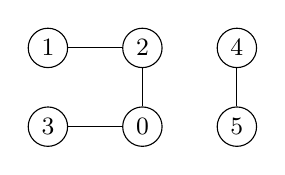
\begin{tikzpicture}
        \node[vertex] (v1) at (0, 1) {1};
        \node[vertex] (v2) at (1.2, 1) {2};
        \node[vertex] (v3) at (0, 0) {3};
        \node[vertex] (v0) at (1.2, 0) {0};
        \node[vertex] (v4) at (2.4, 1) {4};
        \node[vertex] (v5) at (2.4, 0) {5};
        \draw (v1) -- (v2) -- (v0) -- (v3) (v4) -- (v5);
    \end{tikzpicture}}

\begin{document}

% ---------------------------------------------------------------------------
\hypersetup{pageanchor=false}
\begin{titlepage}
    \centering
    \vspace*{5cm}
    {\large\scshape CSESoc Education\par}
    \vspace{1cm}
    {\Huge\bfseries COMP2521\par}
    \vspace{0.4cm}
    {\huge Problem Solving Workshop\par}
    \vspace{0.8cm}
    \rule{0.6\linewidth}{0.8pt}\par
    \vspace{0.8cm}
    {\large Linked Lists \textbullet{} Binary Search Trees \textbullet{} Graphs\par
        Hash Tables \textbullet{} Stacks \& Queues\par}
    \vfill
    \begin{tabular}{l@{\quad}l}
        \level{1} & Easy \\
        \level{2} & Medium \\
        \level{3} & Challenging \\
    \end{tabular}\par
    \vspace{1.5cm}
    \url{https://github.com/itsJae/COMP2521-problem-solving-workshop}
\end{titlepage}
\hypersetup{pageanchor=true}

% ---------------------------------------------------------------------------
\hypertarget{contents}{}
\tableofcontents

% ---------------------------------------------------------------------------
\clearpage
\phantomsection
\addcontentsline{toc}{section}{Getting Started}
\section*{Getting Started}

\heading{Setup}
Install VS Code, Git and a C compiler (see the \texttt{README} for each OS). Then open the Command Palette in VS Code (\texttt{Cmd/Ctrl + Shift + P}), run \textbf{Git: Clone} and paste:
\begin{lstlisting}[language={}]
https://github.com/itsJae/COMP2521-problem-solving-workshop.git
\end{lstlisting}

\heading{Solving a problem}
Each problem is a single C function in its topic folder, for example \texttt{linked\_list/is\_sorted.c}. Fill in the \texttt{TODO}. You may write helper functions, and you may use any ADT in the \texttt{adt/} folder.

\heading{Testing}
Open a terminal in VS Code, move into the topic folder and run \texttt{autotest}:
\begin{lstlisting}[language=bash]
cd linked_list
./autotest is_sorted    # test one problem
./autotest              # test every problem in this folder
\end{lstlisting}
A test fails if your answer is wrong, if your program crashes, or if it takes longer than 5 seconds. Some tests are large, so a solution that is slower than the required time complexity may time out.

To debug with your own \texttt{printf}s, build with \texttt{make} and run the problem directly. This only shows your own output:
\begin{lstlisting}[language=bash]
make
./is_sorted
\end{lstlisting}

\heading{Notation}
In the samples, a linked list is written as \texttt{1 -> 2 -> 3 -> X}, where \texttt{X} is \texttt{NULL}. A BST is given by the order in which values are inserted into an empty tree, together with a drawing of the result.

% ===========================================================================
\topic{Linked List}

\problem{Is Sorted}{1}{linked_list/is_sorted.c}{is_sorted}{$O(n)$}

\heading{Background}
The COMP2521 tutors keep every student's lab mark in a linked list. Their marking script only works if the marks are already in order, so before running it they want a quick check.

\heading{Task}
Return \texttt{true} if the values in the list are in non-decreasing order (every value is less than or equal to the next one), otherwise return \texttt{false}.
\begin{lstlisting}
struct node {
    int value;
    struct node *next;
};

bool isSorted(struct node *list);
\end{lstlisting}

\heading{Assumptions}
\begin{itemize}
    \item The list may be empty (\texttt{NULL}). An empty list and a list with one node are sorted.
    \item You must not use \texttt{for} or \texttt{while} loops. Use recursion instead.
    \item Equal neighbouring values are allowed.
    \item The list must not be modified.
\end{itemize}

\heading{Samples}
\sample{1 -> 2 -> 3 -> 4 -> X}{true}
\sample[\texttt{3} is greater than the next value \texttt{1}.]{3 -> 1 -> 2 -> 4 -> X}{false}

% ---------------------------------------------------------------------------
\problem{Copy Alternating Range}{2}{linked_list/copy_alternating_range.c}{copy_alternating_range}{$O(n)$}

\heading{Background}
Your playlist is a linked list where each node holds a song's energy level. Tonight you only want songs with energy between \texttt{lo} and \texttt{hi}, and to keep things fresh you skip every second song that qualifies.

\heading{Task}
Considering only the values that lie in the inclusive range $[lo, hi]$, return a \textbf{new} list containing the 1st, 3rd, 5th, \ldots{} of them, in their original order.
\begin{lstlisting}
struct node {
    int value;
    struct node *next;
};

struct node *copyAlternatingRange(struct node *list, int lo, int hi);
\end{lstlisting}

\heading{Assumptions}
\begin{itemize}
    \item $lo \le hi$.
    \item The list may be empty. If no value lies in the range, return \texttt{NULL}.
    \item The new list must be built from newly allocated nodes. The original list must not be modified.
\end{itemize}

\heading{Samples}
\sample[The values in {$[3, 8]$} are \texttt{8, 3, 6, 7, 5, 4}. The 1st, 3rd and 5th of them are \texttt{8, 6, 5}.]
    {8 -> 3 -> 6 -> 2 -> 7 -> 5 -> 9 -> 4 -> X \\ lo = 3, hi = 8}
    {8 -> 6 -> 5 -> X}
\sample[Only \texttt{4} and \texttt{6} are in range, and \texttt{6} is the 2nd of them.]
    {10 -> 4 -> 20 -> 6 -> X \\ lo = 4, hi = 6}
    {4 -> X}

% ---------------------------------------------------------------------------
\problem{Delete Mid}{3}{linked_list/delete_mid.c}{delete_mid}{$O(n)$}

\heading{Background}
The waiting line for the CSESoc pubcrawl at Sanctuary Hotel is getting too long. Whoever is standing in the exact middle has been chosen to leave and grab more snacks.

\heading{Task}
Delete the middle node of the list and return the head of the updated list. For a list of length $n$, the middle node is the one at index $\lfloor n/2 \rfloor$, counting from 0.
\begin{lstlisting}
struct node {
    int value;
    struct node *next;
};

struct node *deleteMid(struct node *list);
\end{lstlisting}

\heading{Assumptions}
\begin{itemize}
    \item The list is not empty ($n \ge 1$). If it has one node, the result is \texttt{NULL}.
    \item The deleted node must be freed.
\end{itemize}

\heading{Samples}
\sample[$n = 5$, so the node at index 2 (\texttt{5}) is deleted.]
    {1 -> 3 -> 5 -> 7 -> 9 -> X}{1 -> 3 -> 7 -> 9 -> X}
\sample[$n = 4$, so the node at index 2 (\texttt{3}) is deleted.]
    {1 -> 2 -> 3 -> 4 -> X}{1 -> 2 -> 4 -> X}

% ===========================================================================
\topic{Binary Search Tree}

\problem{Count Leaves}{1}{bst/count_leaves.c}{count_leaves}{$O(n)$}

\heading{Background}
Autumn has arrived on the library lawn, and the BST growing there is about to drop its leaves. Before the gardeners show up, they want to know how many leaves to expect.

\heading{Task}
Return the number of leaf nodes (nodes with no children) in the given BST.
\begin{lstlisting}
struct node {
    int value;
    struct node *left;
    struct node *right;
};

int countLeaves(struct node *tree);
\end{lstlisting}

\heading{Assumptions}
\begin{itemize}
    \item The tree may be empty, in which case there are 0 leaves.
    \item A tree with a single node has 1 leaf.
\end{itemize}

\heading{Samples}
\sample[The leaves are \texttt{1}, \texttt{3} and \texttt{5}.]
    {insert 4 2 6 1 3 5 \par\medskip
     \centering
     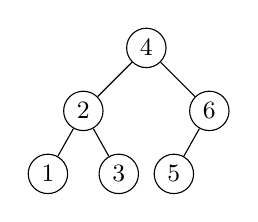
\begin{tikzpicture}[tree]
        \node {4}
            child {node {2} child {node {1}} child {node {3}}}
            child {node {6} child {node {5}} child[missing]};
     \end{tikzpicture}}
    {3}
\sample[The tree is a single path, so \texttt{4} is the only leaf.]
    {insert 1 2 3 4 \par\medskip
     \centering
     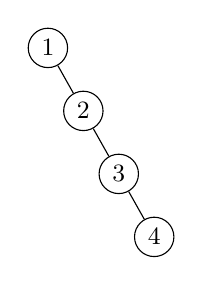
\begin{tikzpicture}[tree, level 1/.style={sibling distance=9mm},
                         level 2/.style={sibling distance=9mm},
                         level 3/.style={sibling distance=9mm}]
        \node {1}
            child[missing]
            child {node {2}
                child[missing]
                child {node {3}
                    child[missing]
                    child {node {4}}}};
     \end{tikzpicture}}
    {1}

% ---------------------------------------------------------------------------
\problem{Tree Diameter}{2}{bst/tree_diameter.c}{tree_diameter}{$O(n)$}

\heading{Background}
A squirrel lives in the library BST. It wants to plan the longest possible trip between two nodes without visiting any node twice.

\heading{Task}
Return the diameter of the tree: the number of \textbf{edges} on the longest path between any two nodes.
\begin{lstlisting}
struct node {
    int value;
    struct node *left;
    struct node *right;
};

int treeDiameter(struct node *tree);
\end{lstlisting}

\heading{Assumptions}
\begin{itemize}
    \item The tree may be empty. An empty tree and a tree with one node both have diameter 0.
    \item The longest path does not have to pass through the root.
\end{itemize}

\heading{Samples}
\sample[The path \texttt{1-2-4-5-6-7} has 5 edges and goes through the root.]
    {insert 5 4 2 1 3 6 7 \par\medskip
     \centering
     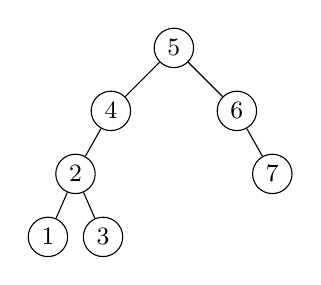
\begin{tikzpicture}[tree]
        \node {5}
            child {node {4} child {node {2} child {node {1}} child {node {3}}} child[missing]}
            child {node {6} child[missing] child {node {7}}};
     \end{tikzpicture}}
    {5}
\sample[The path \texttt{1-2-3-6-4-5} has 5 edges and does not go through the root.]
    {insert 7 3 2 1 6 4 5 8 \par\medskip
     \centering
     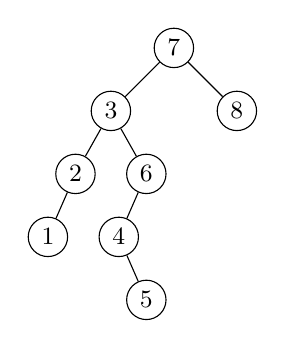
\begin{tikzpicture}[tree]
        \node {7}
            child {node {3}
                child {node {2} child {node {1}} child[missing]}
                child {node {6} child {node {4} child[missing] child {node {5}}} child[missing]}}
            child {node {8}};
     \end{tikzpicture}}
    {5}

% ---------------------------------------------------------------------------
\problem{Structural Difference}{3}{bst/structural_difference.c}{structural_difference}{$O(n + m)$, where $n$ and $m$ are the numbers of nodes in the two trees}

\heading{Background}
Two students submitted BSTs for the same lab exercise. Their tutor plays spot the difference to measure how far apart the two trees are.

\heading{Task}
For every position that occurs in at least one of the two trees:
\begin{itemize}
    \setlength{\itemsep}{0pt}
    \item add 0 if both trees have a node there and the values are equal,
    \item add 1 if both trees have a node there but the values are different,
    \item add 2 if exactly one tree has a node there.
\end{itemize}
Return the total.
\begin{lstlisting}
int structuralDifference(struct node *t1, struct node *t2);
\end{lstlisting}

\heading{Assumptions}
\begin{itemize}
    \item A position is the path of left/right moves from the root, not a value.
    \item Either tree, or both, may be empty.
    \item If one tree has a whole subtree where the other tree has no node, every node in that subtree adds 2.
\end{itemize}

\heading{Samples}
\sample[Root \texttt{8 = 8} adds 0, \texttt{3} vs \texttt{4} adds 1, \texttt{1} and \texttt{14} each exist in only one tree and add 2.]
    {t1: insert 8 3 10 14 \\ t2: insert 8 4 10 1 \par\medskip
     \centering
     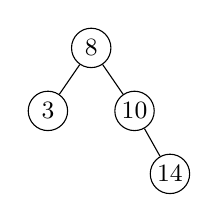
\begin{tikzpicture}[tree, baseline=(current bounding box.center),
                         level 1/.style={sibling distance=11mm}]
        \node {8}
            child {node {3}}
            child {node {10} child[missing] child {node {14}}};
     \end{tikzpicture}
     \quad\textrm{vs}\quad
     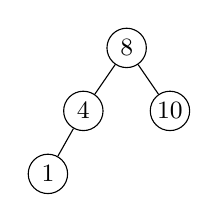
\begin{tikzpicture}[tree, baseline=(current bounding box.center),
                         level 1/.style={sibling distance=11mm}]
        \node {8}
            child {node {4} child {node {1}} child[missing]}
            child {node {10}};
     \end{tikzpicture}}
    {5}
\sample[\texttt{t1} is empty, so all 3 nodes of \texttt{t2} add 2 each.]
    {t1: (empty) \\ t2: insert 2 1 3 \par\medskip
     \centering
     \texttt{X}
     \quad\textrm{vs}\quad
     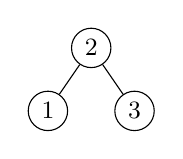
\begin{tikzpicture}[tree, baseline=(current bounding box.center),
                         level 1/.style={sibling distance=11mm}]
        \node {2} child {node {1}} child {node {3}};
     \end{tikzpicture}}
    {6}

% ===========================================================================
\topic{Graph Traversal}

\problem{Reach Darling Square}{1}{graph/reach_darling_square.c}{reach_darling_square}{$O(V + E)$}

\heading{Background}
You and your friends are meeting for dinner at Darling Square. The city is a graph: each vertex is a location and each edge is a direct route between two locations. Before you leave, you want to know whether you can get there at all.

\heading{Task}
Return \texttt{true} if \texttt{dest} (the darling square) can be reached from \texttt{src}, otherwise return \texttt{false}.
\begin{lstlisting}
bool reachDarlingSquare(Graph g, int src, int dest);

// Useful ADT functions
int GraphNumVertices(Graph g);
int GraphDegree(Graph g, int v);
int GraphNeighbour(Graph g, int v, int i);   // 0 <= i < GraphDegree(g, v)

Queue QueueNew(void);
void QueueEnqueue(Queue q, void *item);
void *QueueDequeue(Queue q);
bool QueueIsEmpty(Queue q);
void QueueFree(Queue q, void (*freeItem)(void *item));
\end{lstlisting}

\heading{Assumptions}
\begin{itemize}
    \item The graph is undirected and may be disconnected. Vertices are numbered $0$ to $V - 1$.
    \item $0 \le src, dest < V$. If $src = dest$, the answer is \texttt{true}.
\end{itemize}

\heading{Samples}
Both samples use this graph:
\begin{center}\sampleGraph\end{center}
\sample[\texttt{1 - 2 - 0 - 3} is a path from 1 to 3.]
    {V = 6 \\ edges: 1-2 2-0 0-3 4-5 \\ src = 1, dest = 3}{true}
\sample[Vertex 5 is in a different component from vertex 1.]
    {V = 6 \\ edges: 1-2 2-0 0-3 4-5 \\ src = 1, dest = 5}{false}

% ---------------------------------------------------------------------------
\problem{Find Happy Component}{2}{graph/find_happy_component.c}{find_happy_component}{$O(V + E)$}

\heading{Background}
At the end-of-term party, people cluster into friend groups: two people are in the same group if they are connected by a chain of friendships. A group is only happy if it is big enough.

\heading{Task}
A connected component is \emph{happy} if and only if it has at least $k$ vertices. Return how many components of the graph are happy.
\begin{lstlisting}
int findHappyComponent(Graph g, int k);

// Useful ADT functions
int GraphNumVertices(Graph g);
int GraphDegree(Graph g, int v);
int GraphNeighbour(Graph g, int v, int i);   // 0 <= i < GraphDegree(g, v)

Stack StackNew(void);
void StackPush(Stack s, void *item);
void *StackPop(Stack s);
bool StackIsEmpty(Stack s);
void StackFree(Stack s, void (*freeItem)(void *item));
\end{lstlisting}

\heading{Assumptions}
\begin{itemize}
    \item The graph is undirected. A vertex with no edges is a component of size 1.
    \item $k \ge 1$.
\end{itemize}

\heading{Samples}
Both samples use this graph:
\begin{center}\sampleGraph\end{center}
\sample[The components have sizes 4 and 2. Only the first has at least 3 vertices.]
    {V = 6 \\ edges: 1-2 2-0 0-3 4-5 \\ k = 3}{1}
\sample[Both components have at least 2 vertices.]
    {V = 6 \\ edges: 1-2 2-0 0-3 4-5 \\ k = 2}{2}

% ---------------------------------------------------------------------------
\problem{Celebrity}{3}{graph/celebrity.c}{celebrity}{$O(n)$}

\heading{Background}
Rumour has it that a celebrity has sneaked into the party. Everyone knows the celebrity, but the celebrity does not know anyone. You may only ask questions of the form ``does person $i$ know person $j$?''.
Based on \href{https://www.geeksforgeeks.org/problems/the-celebrity-problem/1}{The Celebrity Problem}.

\heading{Task}
There are $n$ people at the party, and \texttt{mat[i][j] == 1} if person $i$ knows person $j$. A \emph{celebrity} is known by everyone else but knows no one else. Return the index of the celebrity, or $-1$ if there is none.
\begin{lstlisting}
int celebrity(int n, int mat[n][n]);
\end{lstlisting}

\heading{Assumptions}
\begin{itemize}
    \item $n \ge 1$. A party with one person has that person as the celebrity.
    \item \texttt{mat[i][i]} may be 0 or 1 and should be ignored.
    \item Reading the whole matrix takes $O(n^2)$, so you must skip most of it. Hint: each question rules out one person.
\end{itemize}

\heading{Samples}
\sample[Everyone knows person 1, and person 1 knows no one.]
    {n = 3 \\ mat: \\ 0 1 0 \\ 0 0 0 \\ 0 1 0}{1}
\sample[Persons 0 and 1 know each other, so neither is a celebrity.]
    {n = 2 \\ mat: \\ 0 1 \\ 1 0}{-1}

% ===========================================================================
\topic{Hash Table}

\problem{Molly Tea}{1}{hashmap/molly_tea.c}{molly_tea}{$O(n)$ on average}

\heading{Background}
James is a poor uni student on a first date with Julia. He takes her to Molly Tea, opens his wallet, and finds exactly $k$ dollars. He wants to buy two drinks that add up to exactly $k$ dollars so he can spend every last dollar to impress her. Julia gets impatient if James takes too long.

\heading{Task}
Given the drink prices, find two different drinks whose prices add up to exactly $k$. If they exist, store their indices in \texttt{*i} and \texttt{*j} and return \texttt{true}. Otherwise return \texttt{false}.
\begin{lstlisting}
bool mollyTea(int prices[], int n, int k, int *i, int *j);

// Useful ADT functions (see Common.h for HashInt and EqualsInt)
HashTable HashTableNew(HashFn hash, EqualsFn equals);
void HashTablePut(HashTable t, void *key, void *value);
void *HashTableGet(HashTable t, void *key);   // NULL if absent
void HashTableFree(HashTable t, void (*freeKey)(void *key),
                   void (*freeValue)(void *value));
\end{lstlisting}

\heading{Assumptions}
\begin{itemize}
    \item $n \ge 0$. Two different drinks may have the same price, but one drink cannot be bought twice.
    \item If several pairs work, any one of them is accepted.
\end{itemize}

\heading{Samples}
\sample[$2 + 7 = 9$.]
    {prices = [2, 7, 11, 15] \\ k = 9}{true \\ i = 0, j = 1}
\sample[$3 + 3 = 6$, but there is only one drink that costs 3.]
    {prices = [3, 4] \\ k = 6}{false}

% ---------------------------------------------------------------------------
\problem{Isomorphic Strings}{2}{hashmap/isomorphic_strings.c}{isomorphic_strings}{$O(n)$ on average}

\heading{Background}
Your friend sends you a secret message \texttt{t} and claims it is the word \texttt{s} encrypted with a substitution cipher, where each letter is always swapped for the same letter. Before you start decoding, check whether that is even possible.
Based on \href{https://leetcode.com/problems/isomorphic-strings/}{LeetCode 205}.

\heading{Task}
Two strings $s$ and $t$ are isomorphic if the characters in $s$ can be replaced to get $t$, where every occurrence of a character is replaced with the same character, and no two different characters map to the same character. Return \texttt{true} if $s$ and $t$ are isomorphic.
\begin{lstlisting}
bool isIsomorphic(char *s, char *t);
\end{lstlisting}

\heading{Assumptions}
\begin{itemize}
    \item $s$ and $t$ have the same length $n$, which may be 0. Two empty strings are isomorphic.
    \item The strings contain ASCII characters. A character may map to itself.
\end{itemize}

\heading{Samples}
\sample[\texttt{e} maps to \texttt{a} and \texttt{g} maps to \texttt{d}.]
    {s = "egg" \\ t = "add"}{true}
\sample[Both \texttt{b} and \texttt{d} would have to map to \texttt{b}.]
    {s = "badc" \\ t = "baba"}{false}

% ---------------------------------------------------------------------------
\problem{Longest Substring Without Repeating Characters}{3}{hashmap/longest_substring.c}{longest_substring}{$O(n)$ on average}

\heading{Background}
Your music history is a string where each character is a song. You want to brag about your longest listening streak without a single repeat.
Based on \href{https://leetcode.com/problems/longest-substring-without-repeating-characters/}{LeetCode 3}.

\heading{Task}
Return the length of the longest substring of $s$ that contains no repeated characters.
\begin{lstlisting}
int lengthOfLongestSubstring(char *s);
\end{lstlisting}

\heading{Assumptions}
\begin{itemize}
    \item $s$ may be empty, in which case the answer is 0.
    \item $s$ contains ASCII characters, including spaces.
    \item A substring is contiguous: \texttt{"pwke"} is not a substring of \texttt{"pwwkew"}.
\end{itemize}

\heading{Samples}
\sample[The longest such substring is \texttt{"abc"}.]
    {s = "abcabcbb"}{3}
\sample[The longest such substring is \texttt{"wke"}.]
    {s = "pwwkew"}{3}

% ===========================================================================
\topic{Stack / Queue}

\problem{Crunch Pringles}{1}{stack_queue/crunch_pringles.c}{crunch_pringles}{$O(n^2)$}

\heading{Background}
A Pringles tube only opens at the top, so it behaves like a stack. Each chip has an integer crunch score, and you want to save the crunchiest chip for last.

\heading{Task}
Sort the tube in place so that scores never decrease from bottom to top (the crunchiest chip ends up on top). You may use \texttt{bowl}, an empty stack, as temporary storage.
\begin{lstlisting}
void sortTube(Stack tube, Stack bowl);

// Useful ADT functions (every item is an int *)
void StackPush(Stack s, void *item);
void *StackPop(Stack s);
void *StackPeek(Stack s);
bool StackIsEmpty(Stack s);
\end{lstlisting}

\heading{Assumptions}
\begin{itemize}
    \item The tube may be empty. Scores may be negative or repeated.
    \item Apart from the two stacks, use only a constant number of variables (no arrays or other ADTs).
    \item Move the existing items. Do not allocate new ones.
\end{itemize}

\heading{Samples}
\sample{tube (bottom -> top): \\ 3 1 4 2}{tube (bottom -> top): \\ 1 2 3 4}
\sample{tube (bottom -> top): \\ 5 5 2}{tube (bottom -> top): \\ 2 5 5}

% ---------------------------------------------------------------------------
\problem{Reverse Queue}{2}{stack_queue/reverse_queue.c}{reverse_queue}{$O(n)$}

\heading{Background}
It is happy hour at the food court, and the manager announces that whoever joined the queue last will be served first.

\heading{Task}
Reverse the order of the items in the queue in place, so the item at the back ends up at the front.
\begin{lstlisting}
void reverseQueue(Queue q);

// Useful ADT functions (every item is an int *)
void QueueEnqueue(Queue q, void *item);
void *QueueDequeue(Queue q);
bool QueueIsEmpty(Queue q);

Stack StackNew(void);
void StackPush(Stack s, void *item);
void *StackPop(Stack s);
bool StackIsEmpty(Stack s);
void StackFree(Stack s, void (*freeItem)(void *item));
\end{lstlisting}

\heading{Assumptions}
\begin{itemize}
    \item The queue may be empty. Values may be repeated.
    \item Move the existing items. Do not allocate new ones.
\end{itemize}

\heading{Samples}
\sample{q (front -> back): \\ 1 2 3 4 5}{q (front -> back): \\ 5 4 3 2 1}
\sample{q (front -> back): \\ 3 3 1}{q (front -> back): \\ 1 3 3}

% ---------------------------------------------------------------------------
\problem{Daily Temperatures}{3}{stack_queue/daily_temperatures.c}{daily_temperatures}{$O(n)$}

\heading{Background}
Sydney weather is unpredictable, and you are planning your beach days. For every day, you want to know how long you would have to wait for a warmer one.
Based on \href{https://leetcode.com/problems/daily-temperatures/}{LeetCode 739}.

\heading{Task}
\texttt{temperatures[i]} is the temperature on day $i$. For each day, set \texttt{answer[i]} to the number of days you have to wait after day $i$ to get a warmer temperature, or $0$ if there is no such day.
\begin{lstlisting}
void dailyTemperatures(int temperatures[], int n, int answer[]);
\end{lstlisting}

\heading{Assumptions}
\begin{itemize}
    \item $0 \le n \le 200\,000$, and \texttt{answer} has room for $n$ values.
    \item An equal temperature is not warmer.
    \item An $O(n^2)$ solution is too slow for the largest test. Hint: a stack of days that are still waiting for a warmer day.
\end{itemize}

\heading{Samples}
\sample[Day 2 (\texttt{75}) waits until day 6 (\texttt{76}), so {\texttt{answer[2] = 4}}.]
    {temperatures = \\ {[}73, 74, 75, 71, 69, 72, 76, 73{]}}{answer = \\ {[}1, 1, 4, 2, 1, 1, 0, 0{]}}
\sample{temperatures = \\ {[}30, 40, 50, 60{]}}{answer = \\ {[}1, 1, 1, 0{]}}

% ===========================================================================
\topic{Bonus}

\problem{Project Selection}{3}{bonus/project_selection.c}{project_selection}{$O(n \log k)$}

\heading{Background}
You are planning your degree. Each project needs some knowledge before you can start it, and teaches you more once you finish. You only have time for $k$ projects, so choose wisely.

\heading{Task}
You are given two arrays \texttt{R} and \texttt{W}, and two other inputs $s$ and $k$:
\begin{itemize}
    \setlength{\itemsep}{0pt}
    \item \texttt{R[i]} is the knowledge required to select project $i$,
    \item \texttt{W[i]} is the knowledge gained after selecting project $i$,
    \item $s$ is your starting knowledge, and $k$ is the number of projects to select.
\end{itemize}
Your knowledge grows by \texttt{W[i]} after each project you select, and you cannot select the same project twice.

\textbf{(a)} Which data structure solves the problem in $O(n \log k)$ time?
\begin{enumerate}[label=\Alph*., itemsep=0pt, parsep=0pt]
    \item Stack
    \item Queue
    \item Unordered array
    \item AVL tree
    \item Heap
\end{enumerate}

\textbf{(b)} Return the maximum knowledge you can have after selecting $k$ projects.
\begin{lstlisting}
int projectSelection(int R[], int W[], int n, int s, int k);
\end{lstlisting}

\heading{Assumptions}
\begin{itemize}
    \item \texttt{R} is sorted in ascending order.
    \item $1 \le k \le n$, and it is always possible to select $k$ projects.
\end{itemize}

\heading{Samples}
\sample[Select projects 1, 4 and 3: $2 \to 5 \to 15 \to 19$.]
    {R = [1, 2, 2, 3, 4] \\ W = [2, 3, 1, 4, 10] \\ s = 2, k = 3}{19}
\sample[Select projects 0, 2 and 3: $0 \to 5 \to 15 \to 17$.]
    {R = [0, 2, 5, 10] \\ W = [5, 1, 10, 2] \\ s = 0, k = 3}{17}

\end{document}
